\chapter{Fault Characterization and Observation}
\label{chap:fault-model}

Persistent faults in static memory are the central concern of this work. 
Transient faults that arise in dynamic elements—such as registers, caches, or SRAM—are short-lived and typically disappear after a reset or rewrite. 
In these cases, detection and restart are sufficient to restore correct operation. 
In contrast, \textbf{static memory}—such as flash, ROM, EEPROM, or other non-volatile storage—retains errors across resets and power cycles. 
A corrupted instruction or data word in these regions permanently alters program behavior, making persistence rather than transience the defining property of the reliability challenge.




Figure~\ref{fig:system-diagram} illustrates a representative embedded microcontroller architecture.
The CPU serves as the execution core, surrounded by memory and peripheral subsystems. 
Program memory contains the executable instructions that define control flow, while RAM stores transient computation state. 
EEPROM often holds configuration or calibration data that is written infrequently but read frequently.
From a reliability perspective, these three types of memory exhibit distinct fault behavior. 
RAM faults are ephemeral and can usually be cleared through reset, whereas EEPROM and flash-based program memory retain corruption indefinitely.
This persistence makes them the dominant source of long-term reliability degradation in embedded devices.

\begin{figure}[t]
  \centering
  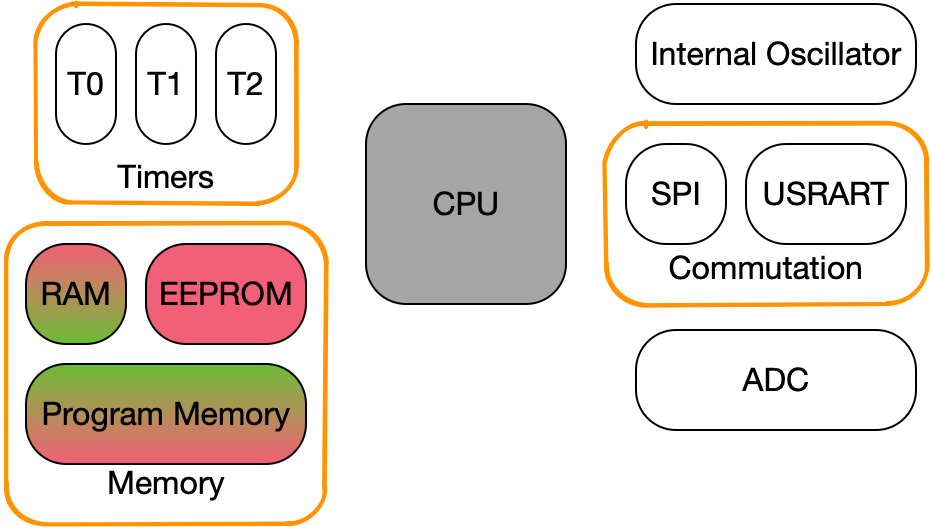
\includegraphics[width=0.85\linewidth]{Chapter-2/figs/system-diagram.png}
  \caption{
  Simplified microcontroller architecture highlighting major subsystems where faults may arise.
  The CPU interfaces with three key memory components: volatile \textbf{RAM}, semi-persistent \textbf{EEPROM}, 
  and non-volatile \textbf{program memory} (typically flash or ROM). 
  Peripheral units such as timers, communication interfaces (SPI, USART), and the ADC rely on correct instruction and data delivery from these memories.
  Transient faults primarily affect dynamic regions such as RAM or registers, while faults in EEPROM or flash persist across reboots, directly threatening long-term system reliability.
  }
  \label{fig:system-diagram}
\end{figure}

\section{Overview of Fault Types}
\label{sec:fault-types}

Faults in computing systems can be grouped by duration and repeatability:

\begin{itemize}
  \item \textbf{Transient faults} are short-lived disturbances caused by radiation, voltage fluctuations, or environmental interference. They affect the current state but vanish after a reset or overwrite.
  \item \textbf{Intermittent faults} recur under specific operational or environmental conditions—such as temperature or voltage stress—but are not permanently fixed in hardware.
  \item \textbf{Persistent faults} alter the stored representation of the program or data. They remain present until the affected memory is explicitly rewritten or replaced.
\end{itemize}

While transient and intermittent faults degrade runtime stability, persistent faults have far more severe implications for embedded and long-lived systems. 
They can render a device permanently unreliable, even when transient protection mechanisms such as ECC, replay, or watchdog recovery are active.

\section{Fault Localization in the Memory Hierarchy}
\label{sec:fault-localization}

The likelihood and impact of faults vary with their position in the memory hierarchy. 
Dynamic memories such as SRAM hold ephemeral runtime data, while non-volatile storage retains the permanent program image. 
Static regions—including \texttt{.text}, \texttt{.rodata}, and the pre-initialized portion of \texttt{.data}—are loaded or executed directly from persistent memory. 
Any corruption in these sections introduces \textbf{deterministic faults}: each fetch or load reproduces the same error on every execution.

By contrast, transient upsets in volatile state—such as a flipped register bit—are naturally overwritten during program progress and rarely persist. 
This distinction makes static instruction and data segments the dominant risk surface for persistent reliability failures.

\section{Statistical Fault Model}
\label{sec:statistical-model}

We model reliability beginning at the cell level. 
Let $p_f$ denote the probability that a single memory cell is faulty, with faults assumed to occur independently across cells. 
For a memory block containing $M$ cells, the probability that the entire block is fault-free is:

\begin{equation}
p_{\mathrm{free}} = (1 - p_f)^M
\end{equation}

The complementary probability that the block contains at least one fault is:

\begin{equation}
p_{\mathrm{fail}} = 1 - (1 - p_f)^M
\end{equation}

This relationship shows the exponential sensitivity of reliability to block size. 
Even when $p_f$ is extremely small, increasing $M$ rapidly reduces the chance that the entire block remains fault-free. 
For small $p_f$, the approximation $p_{\mathrm{fail}} \approx M \cdot p_f$ reveals the linear dependence of failure likelihood on block size in the low-fault regime.

\begin{figure}[t]
  \centering
  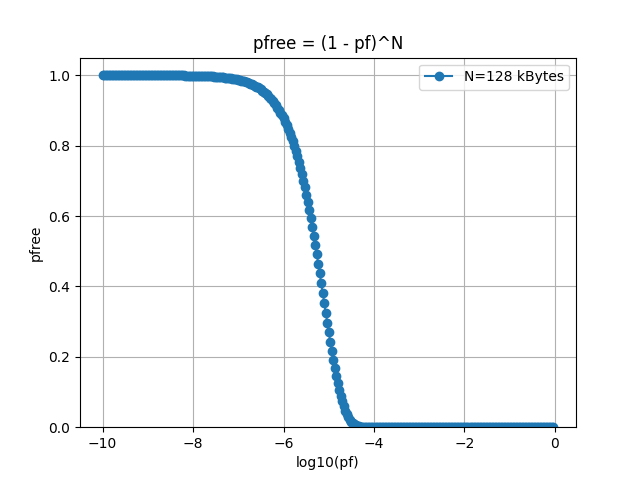
\includegraphics[width=0.90\linewidth]{Chapter-2/figs/pfree.png}
  \caption{System survival probability $p_{\mathrm{free}}$ versus per-cell fault probability $p_f$ for a 128~kB memory region. 
  The logarithmic scale highlights the sharp reliability collapse as $p_f$ increases beyond $10^{-8}$.}
  \label{fig:pfree}
\end{figure}

When plotted for a 128~kB region, reliability remains nearly perfect while $p_f$ is below about $10^{-10}$, but collapses rapidly once $p_f$ rises beyond $10^{-8}$. 
By $10^{-4}$, the chance of a fault-free region is effectively zero. 
This steep ``S-curve'' illustrates how even modest increases in bit-error probability can lead to catastrophic unreliability in large memories.

\section{Raw vs. Unrecoverable Error Rates}
\label{sec:raw-vs-uer}

The per-cell probability $p_f$ represents the \textit{raw error rate} of the underlying technology. 
In practice, systems employ multiple layers of mitigation—such as Error-Correcting Codes (ECC), redundancy, or block replacement—that mask or repair many faults before they affect execution. 
The rate that remains after correction is the \textit{unrecoverable error rate (UER)}.

The difference between the raw error rate and the UER reflects the strength of the protection mechanism. 
A robust ECC scheme can tolerate most single-bit and some multi-bit faults, lowering the effective UER by several orders of magnitude. 
Weak or absent protection leaves the UER nearly equal to $p_f$. 
Thus, while the raw error rate gives a device-level measure of reliability, the UER determines the operational reliability of the system as experienced by software.

These models provide the analytical foundation for evaluating how faults in static memory propagate through software systems. 
The next chapter builds on this foundation by examining how an unprotected system behaves under injected faults, establishing a baseline against which repair and replication mechanisms can be measured.